\section{Encuesta}
La herramienta presentada a continuación se realizo en la plataforma Formularios de Google, teniendo en cuenta que el producto planteado es una solución tecnológica y por lo tanto la muestra debería por supuesto tener acceso a la tecnología y ser mayores de edad, con estas dos únicas restricciones se aplico la siguiente encuesta\\
\\
\begin{enumerate}
\item ¿Alguna vez he contratado un servicio de músicos informales?
\item  ¿En el futuro planeo utilizar algún servicio de músicos informales?
\item  ¿Conozco algún artista que necesite promoción?
\item  ¿Conozco alguna plataforma o aplicación de contratación de servicios de músicos informales?
\item  Si la respuesta anterior fue sí, escriba cuál
\item  ¿Utilizó alguna plataforma o aplicación de música o entretenimiento y la tengo configurada a mi gusto?
\item  Si la respuesta anterior fue sí, escriba cual
\item  Cuando contrato un músico informal, me gusta:
    \begin{enumerate}
    \item Contratarlo personalmente
    \item Ver presentaciones anteriores
    \item Saber el costo del servicio
    \item Solo con una recomendación es suficiente
    \item Leer comentarios
    \item Pagar por el servicio en efectivo
    \item Pagar por el servicio con tarjeta
    \end{enumerate}
\item  Si pudiera ver comentarios, vídeos, imágenes y calificación de un grupo o músico informal, ¿lo contrataría a través de una plataforma digital?
    \begin{enumerate}
    \item si
    \item no
    \end{enumerate}
\item  Si la respuesta anterior fue no, escriba las razones
\item  ¿Con qué frecuencia ud. contrata músicos informales para sus eventos?
    \begin{enumerate}
    \item una vez al mes
    \item una vez por trimestre
    \item una vez por semestre
    \item una vez por año
    \item casi nunca
    \end{enumerate}
\end{enumerate}
\section{Tabulación y ordenamiento de información}

\begin{center}
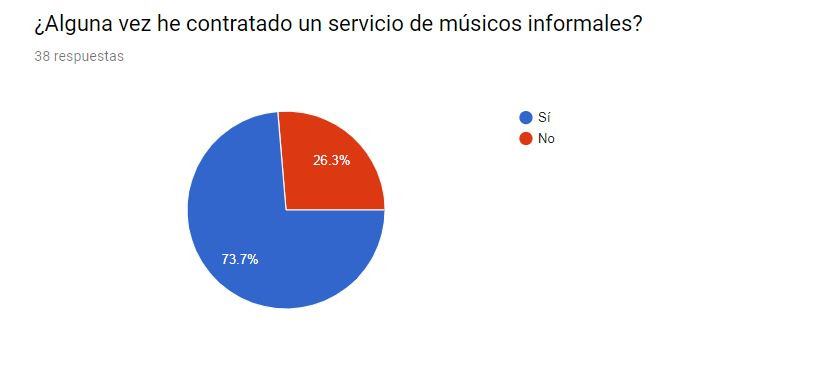
\includegraphics[width=16cm, height=10cm,keepaspectratio=true]{Desarrollo/RecoleccionInformacion/imgs/1.JPG}
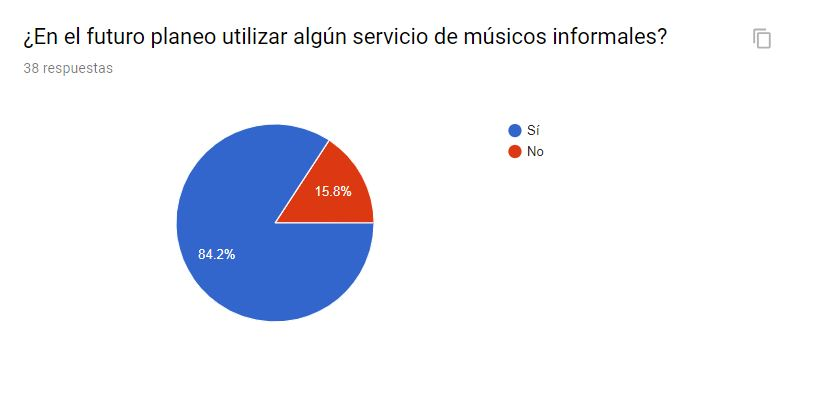
\includegraphics[width=16cm, height=10cm,keepaspectratio=true]{Desarrollo/RecoleccionInformacion/imgs/2.JPG}
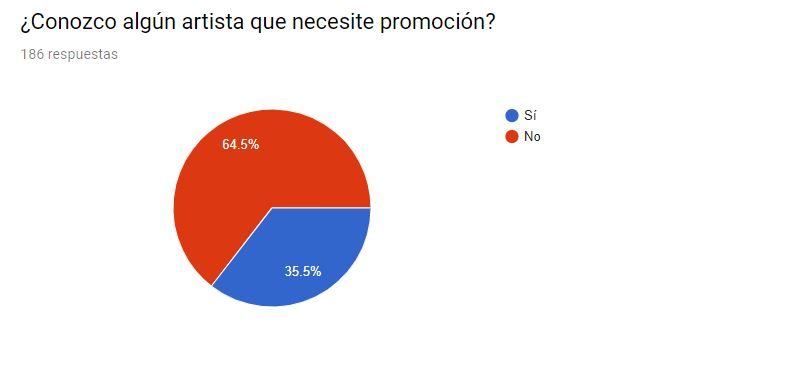
\includegraphics[width=16cm, height=10cm,keepaspectratio=true]{Desarrollo/RecoleccionInformacion/imgs/3.JPG}
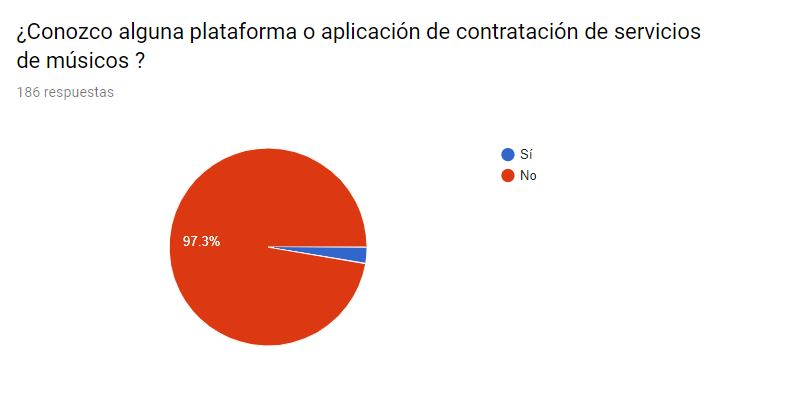
\includegraphics[width=16cm, height=10cm,keepaspectratio=true]{Desarrollo/RecoleccionInformacion/imgs/4.JPG}

\includegraphics[width=16cm, height=10cm,keepaspectratio=true]{Desarrollo/RecoleccionInformacion/imgs/5.JPG}
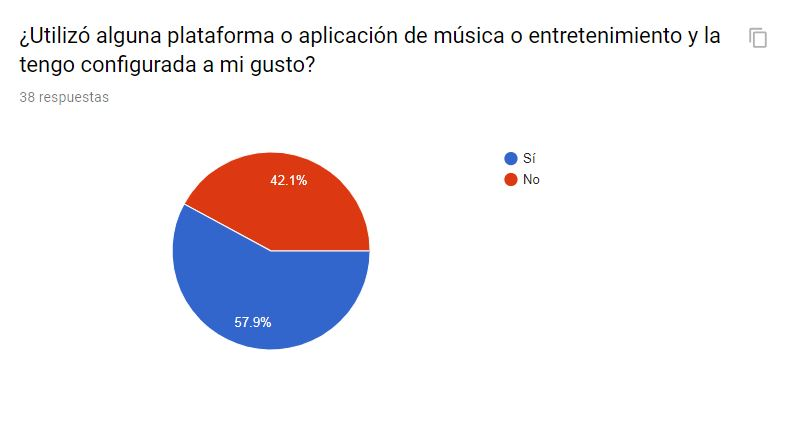
\includegraphics[width=16cm, height=10cm,keepaspectratio=true]{Desarrollo/RecoleccionInformacion/imgs/6.JPG}
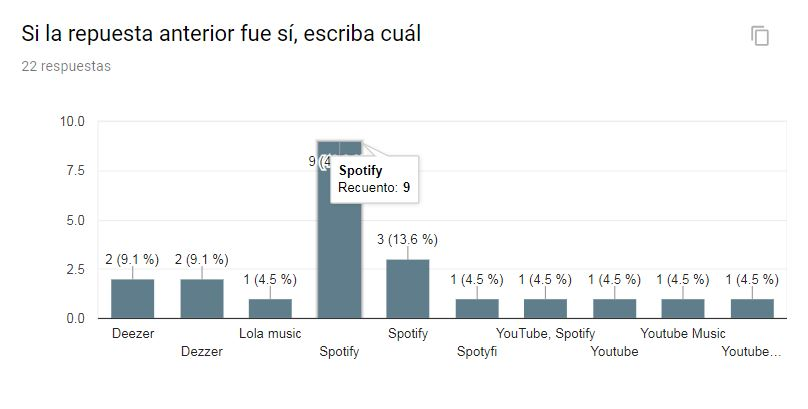
\includegraphics[width=16cm, height=10cm,keepaspectratio=true]{Desarrollo/RecoleccionInformacion/imgs/7.JPG}
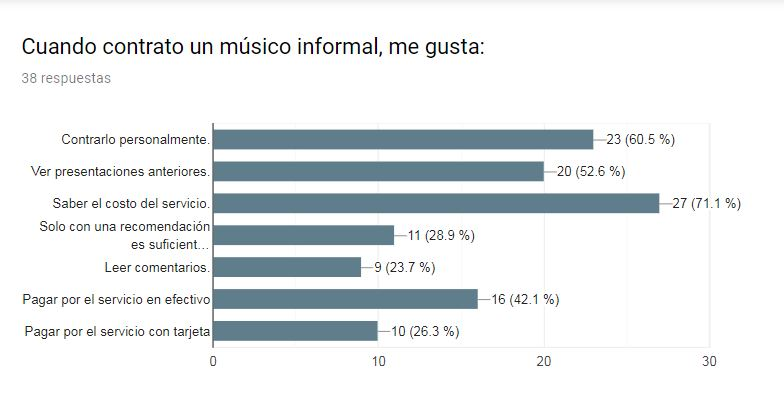
\includegraphics[width=16cm, height=10cm,keepaspectratio=true]{Desarrollo/RecoleccionInformacion/imgs/8.JPG}
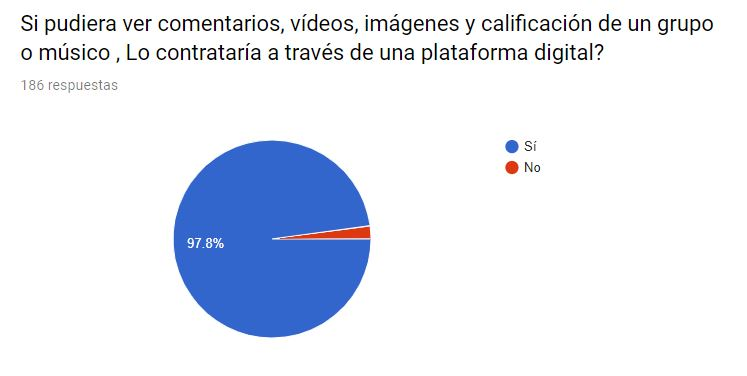
\includegraphics[width=16cm, height=10cm,keepaspectratio=true]{Desarrollo/RecoleccionInformacion/imgs/9.JPG}
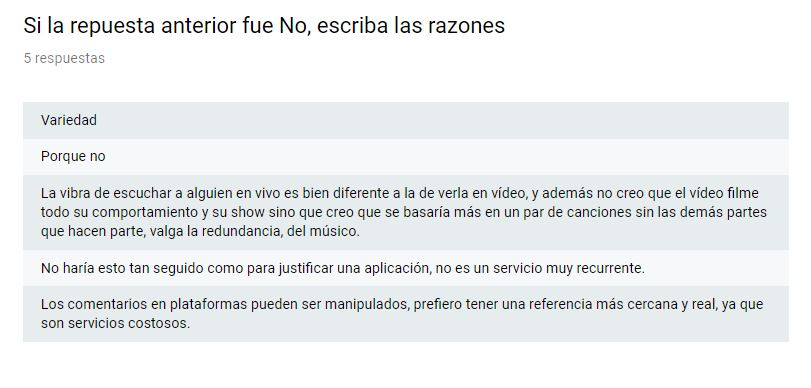
\includegraphics[width=16cm, height=10cm,keepaspectratio=true]{Desarrollo/RecoleccionInformacion/imgs/10.JPG}
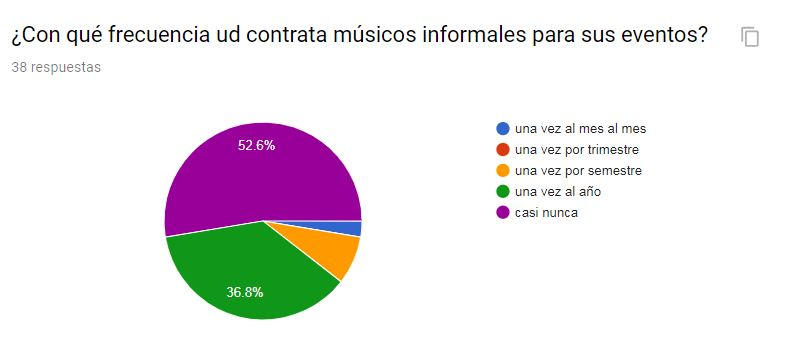
\includegraphics[width=16cm, height=10cm,keepaspectratio=true]{Desarrollo/RecoleccionInformacion/imgs/11.JPG}
\end{center}
\newpage
\section{Análisis de la información}

La muestra tuvo un tamaño de 38 individuos, ordenados en los siguientes grupos:\\
\begin{center}
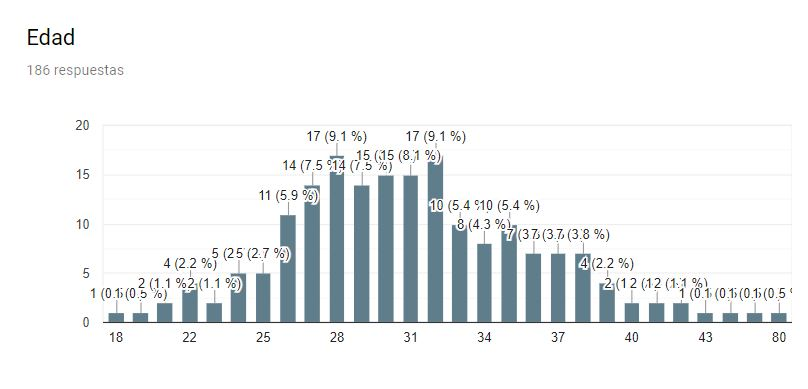
\includegraphics[width=16cm, height=10cm,keepaspectratio=true]{Desarrollo/RecoleccionInformacion/imgs/edad.JPG}
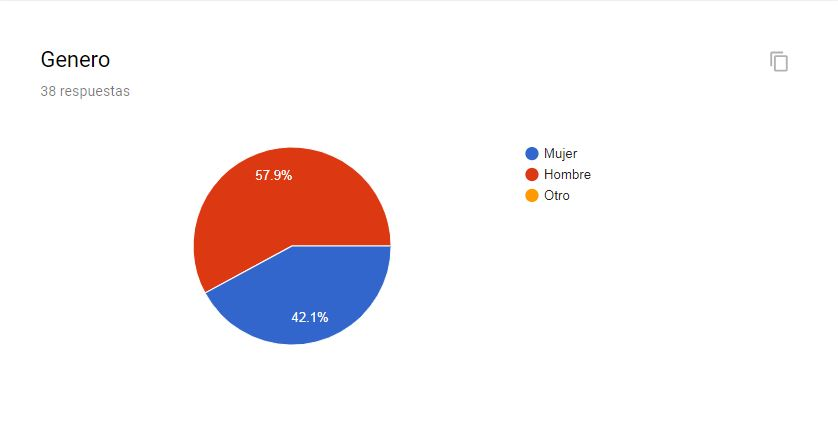
\includegraphics[width=16cm, height=10cm,keepaspectratio=true]{Desarrollo/RecoleccionInformacion/imgs/genero.JPG}
\end{center}
De lo anterior se infiere la viabilidad del proyecto; pues de una muestra variada y posibilitada para utilizarlo, presenta una expectativa de consumo del 97.4 \% \\
Por otro lado el consumo del servicio seria apropiado teniendo en cuenta que para una muestra de este tamaño el 36 \% utiliza los servicios de un músico informal. Y aunque el 52 \% dijo nunca realizar esta actividad se pueden interesar por la reproducción y visualización de medios multimedia como entretenimiento.\\
Se evidencio que en el futuro cercano si existe la posibilidad de realizar la contratación de un musico informal; pero la dificultad o la falta de conocimiento en el proceso disminuye el interés, por lo que la solución planteada debe ser lo mas simple y sencilla y por otro lado como el procedimiento centralizara todo la transcendida se espera gran acogida.
